% Created by tikzDevice version 0.8.1 on 2015-05-24 13:12:08
% !TEX encoding = UTF-8 Unicode
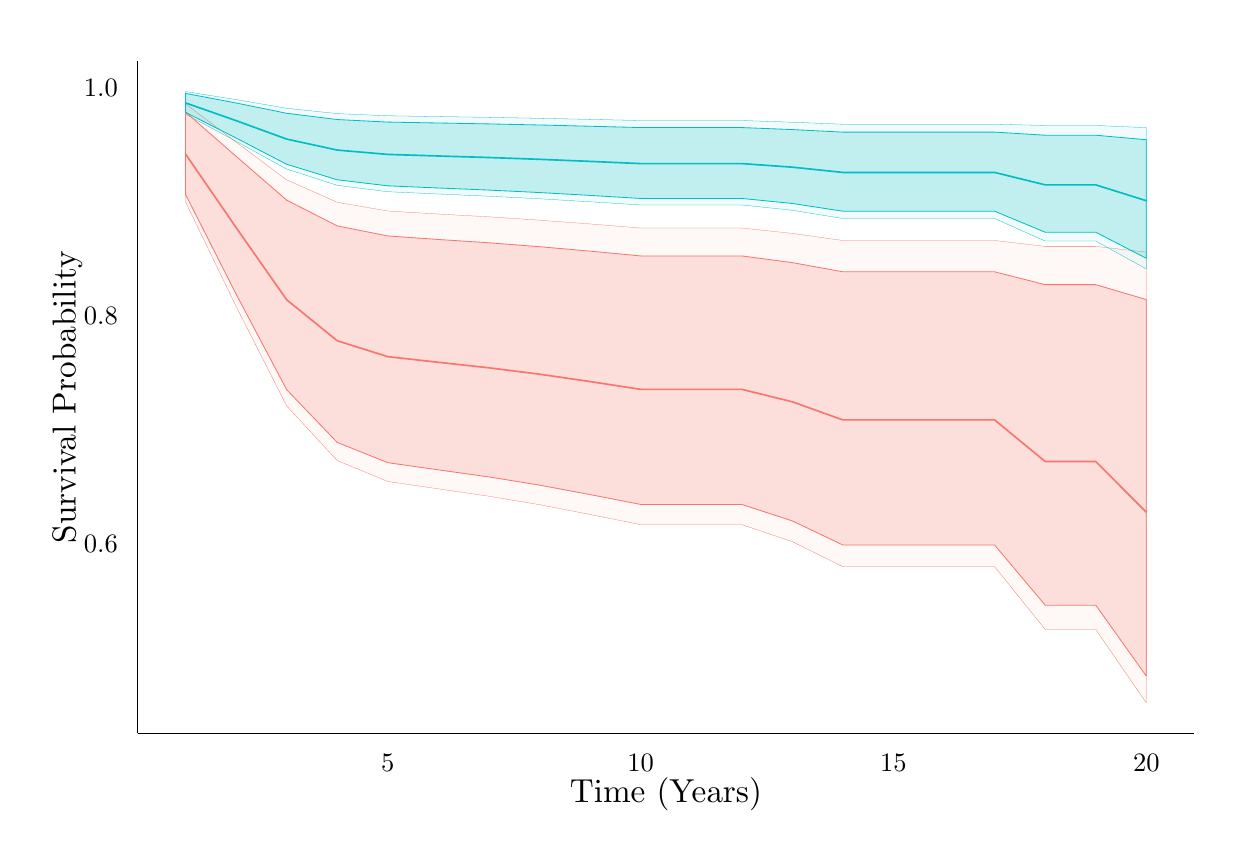
\begin{tikzpicture}[x=1pt,y=1pt]
\definecolor{fillColor}{RGB}{255,255,255}
\path[use as bounding box,fill=fillColor,fill opacity=0.00] (0,0) rectangle (433.62,289.08);
\begin{scope}
\path[clip] (  0.00,  0.00) rectangle (433.62,289.08);
\definecolor{drawColor}{RGB}{255,255,255}
\definecolor{fillColor}{RGB}{255,255,255}

\path[draw=drawColor,line width= 0.6pt,line join=round,line cap=round,fill=fillColor] (  0.00,  0.00) rectangle (433.62,289.08);
\end{scope}
\begin{scope}
\path[clip] ( 39.69, 34.03) rectangle (421.57,277.03);
\definecolor{fillColor}{RGB}{255,255,255}

\path[fill=fillColor] ( 39.69, 34.03) rectangle (421.58,277.03);
\definecolor{drawColor}{RGB}{248,118,109}

\path[draw=drawColor,line width= 0.6pt,line join=round] ( 57.05,243.40) --
	( 75.32,216.83) --
	( 93.59,190.76) --
	(111.86,175.94) --
	(130.13,170.20) --
	(148.41,168.16) --
	(166.68,166.17) --
	(184.95,163.86) --
	(203.22,161.20) --
	(221.49,158.39) --
	(239.77,158.39) --
	(258.04,158.39) --
	(276.31,153.88) --
	(294.58,147.34) --
	(312.86,147.34) --
	(331.13,147.34) --
	(349.40,147.34) --
	(367.67,132.31) --
	(385.94,132.31) --
	(404.22,113.99);
\definecolor{drawColor}{RGB}{0,191,196}

\path[draw=drawColor,line width= 0.6pt,line join=round] ( 57.05,261.89) --
	( 75.32,255.48) --
	( 93.59,248.82) --
	(111.86,244.85) --
	(130.13,243.28) --
	(148.41,242.71) --
	(166.68,242.16) --
	(184.95,241.51) --
	(203.22,240.76) --
	(221.49,239.96) --
	(239.77,239.96) --
	(258.04,239.96) --
	(276.31,238.67) --
	(294.58,236.77) --
	(312.86,236.77) --
	(331.13,236.77) --
	(349.40,236.77) --
	(367.67,232.28) --
	(385.94,232.28) --
	(404.22,226.54);
\definecolor{drawColor}{RGB}{248,118,109}
\definecolor{fillColor}{RGB}{248,118,109}

\path[draw=drawColor,line width= 0.1pt,line join=round,line cap=round,fill=fillColor,fill opacity=0.05] ( 57.05,261.55) --
	( 75.32,247.73) --
	( 93.59,234.09) --
	(111.86,225.99) --
	(130.13,222.84) --
	(148.41,221.73) --
	(166.68,220.73) --
	(184.95,219.52) --
	(203.22,218.16) --
	(221.49,216.68) --
	(239.77,216.68) --
	(258.04,216.68) --
	(276.31,214.74) --
	(294.58,212.17) --
	(312.86,212.17) --
	(331.13,212.17) --
	(349.40,212.17) --
	(367.67,210.05) --
	(385.94,210.05) --
	(404.22,207.96) --
	(404.22, 45.08) --
	(385.94, 71.63) --
	(367.67, 71.63) --
	(349.40, 94.30) --
	(331.13, 94.30) --
	(312.86, 94.30) --
	(294.58, 94.30) --
	(276.31,103.34) --
	(258.04,109.51) --
	(239.77,109.51) --
	(221.49,109.51) --
	(203.22,113.19) --
	(184.95,116.71) --
	(166.68,119.77) --
	(148.41,122.43) --
	(130.13,125.10) --
	(111.86,132.66) --
	( 93.59,152.39) --
	( 75.32,188.37) --
	( 57.05,226.06) --
	cycle;
\definecolor{drawColor}{RGB}{0,191,196}
\definecolor{fillColor}{RGB}{0,191,196}

\path[draw=drawColor,line width= 0.1pt,line join=round,line cap=round,fill=fillColor,fill opacity=0.05] ( 57.05,265.99) --
	( 75.32,263.09) --
	( 93.59,259.95) --
	(111.86,258.03) --
	(130.13,257.24) --
	(148.41,256.95) --
	(166.68,256.67) --
	(184.95,256.33) --
	(203.22,255.94) --
	(221.49,255.53) --
	(239.77,255.53) --
	(258.04,255.53) --
	(276.31,254.91) --
	(294.58,254.19) --
	(312.86,254.19) --
	(331.13,254.19) --
	(349.40,254.19) --
	(367.67,253.74) --
	(385.94,253.74) --
	(404.22,252.95) --
	(404.22,201.88) --
	(385.94,211.98) --
	(367.67,211.98) --
	(349.40,220.12) --
	(331.13,220.12) --
	(312.86,220.12) --
	(294.58,220.12) --
	(276.31,223.10) --
	(258.04,225.01) --
	(239.77,225.01) --
	(221.49,225.01) --
	(203.22,226.16) --
	(184.95,227.24) --
	(166.68,228.17) --
	(148.41,228.98) --
	(130.13,229.80) --
	(111.86,232.10) --
	( 93.59,237.99) --
	( 75.32,248.01) --
	( 57.05,257.84) --
	cycle;
\definecolor{drawColor}{RGB}{248,118,109}
\definecolor{fillColor}{RGB}{248,118,109}

\path[draw=drawColor,line width= 0.3pt,line join=round,line cap=round,fill=fillColor,fill opacity=0.20] ( 57.05,258.58) --
	( 75.32,242.59) --
	( 93.59,226.76) --
	(111.86,217.44) --
	(130.13,213.82) --
	(148.41,212.54) --
	(166.68,211.35) --
	(184.95,209.93) --
	(203.22,208.33) --
	(221.49,206.60) --
	(239.77,206.60) --
	(258.04,206.60) --
	(276.31,204.18) --
	(294.58,200.85) --
	(312.86,200.85) --
	(331.13,200.85) --
	(349.40,200.85) --
	(367.67,196.22) --
	(385.94,196.22) --
	(404.22,190.82) --
	(404.22, 54.77) --
	(385.94, 80.40) --
	(367.67, 80.40) --
	(349.40,102.13) --
	(331.13,102.13) --
	(312.86,102.13) --
	(294.58,102.13) --
	(276.31,110.85) --
	(258.04,116.80) --
	(239.77,116.80) --
	(221.49,116.80) --
	(203.22,120.36) --
	(184.95,123.78) --
	(166.68,126.74) --
	(148.41,129.30) --
	(130.13,131.89) --
	(111.86,139.20) --
	( 93.59,158.25) --
	( 75.32,192.79) --
	( 57.05,228.80) --
	cycle;
\definecolor{drawColor}{RGB}{0,191,196}
\definecolor{fillColor}{RGB}{0,191,196}

\path[draw=drawColor,line width= 0.3pt,line join=round,line cap=round,fill=fillColor,fill opacity=0.20] ( 57.05,265.33) --
	( 75.32,261.86) --
	( 93.59,258.14) --
	(111.86,255.88) --
	(130.13,254.96) --
	(148.41,254.63) --
	(166.68,254.30) --
	(184.95,253.91) --
	(203.22,253.46) --
	(221.49,252.98) --
	(239.77,252.98) --
	(258.04,252.98) --
	(276.31,252.25) --
	(294.58,251.33) --
	(312.86,251.33) --
	(331.13,251.33) --
	(349.40,251.33) --
	(367.67,250.21) --
	(385.94,250.21) --
	(404.22,248.58) --
	(404.22,205.73) --
	(385.94,215.17) --
	(367.67,215.17) --
	(349.40,222.75) --
	(331.13,222.75) --
	(312.86,222.75) --
	(294.58,222.75) --
	(276.31,225.56) --
	(258.04,227.37) --
	(239.77,227.37) --
	(221.49,227.37) --
	(203.22,228.47) --
	(184.95,229.50) --
	(166.68,230.39) --
	(148.41,231.15) --
	(130.13,231.93) --
	(111.86,234.12) --
	( 93.59,239.71) --
	( 75.32,249.20) --
	( 57.05,258.48) --
	cycle;
\end{scope}
\begin{scope}
\path[clip] (  0.00,  0.00) rectangle (433.62,289.08);
\definecolor{drawColor}{RGB}{0,0,0}

\path[draw=drawColor,line width= 0.6pt,line join=round] ( 39.69, 34.03) --
	( 39.69,277.03);
\end{scope}
\begin{scope}
\path[clip] (  0.00,  0.00) rectangle (433.62,289.08);
\definecolor{drawColor}{RGB}{0,0,0}

\node[text=drawColor,anchor=base east,inner sep=0pt, outer sep=0pt, scale=  0.96] at ( 32.57, 99.42) {0.6};

\node[text=drawColor,anchor=base east,inner sep=0pt, outer sep=0pt, scale=  0.96] at ( 32.57,181.75) {0.8};

\node[text=drawColor,anchor=base east,inner sep=0pt, outer sep=0pt, scale=  0.96] at ( 32.57,264.09) {1.0};
\end{scope}
\begin{scope}
\path[clip] (  0.00,  0.00) rectangle (433.62,289.08);
\definecolor{drawColor}{RGB}{0,0,0}

\path[draw=drawColor,line width= 0.6pt,line join=round] ( 39.69, 34.03) --
	(421.57, 34.03);
\end{scope}
\begin{scope}
\path[clip] (  0.00,  0.00) rectangle (433.62,289.08);
\definecolor{drawColor}{RGB}{0,0,0}

\node[text=drawColor,anchor=base,inner sep=0pt, outer sep=0pt, scale=  0.96] at (130.13, 20.31) {5};

\node[text=drawColor,anchor=base,inner sep=0pt, outer sep=0pt, scale=  0.96] at (221.49, 20.31) {10};

\node[text=drawColor,anchor=base,inner sep=0pt, outer sep=0pt, scale=  0.96] at (312.86, 20.31) {15};

\node[text=drawColor,anchor=base,inner sep=0pt, outer sep=0pt, scale=  0.96] at (404.22, 20.31) {20};
\end{scope}
\begin{scope}
\path[clip] (  0.00,  0.00) rectangle (433.62,289.08);
\definecolor{drawColor}{RGB}{0,0,0}

\node[text=drawColor,anchor=base,inner sep=0pt, outer sep=0pt, scale=  1.20] at (230.63,  9.03) {Time (Years)};
\end{scope}
\begin{scope}
\path[clip] (  0.00,  0.00) rectangle (433.62,289.08);
\definecolor{drawColor}{RGB}{0,0,0}

\node[text=drawColor,rotate= 90.00,anchor=base,inner sep=0pt, outer sep=0pt, scale=  1.20] at ( 17.30,155.53) {Survival Probability};
\end{scope}
\end{tikzpicture}
